\RequirePackage[l2tabu, orthodox]{nag}
\documentclass[12pt,a4paper]{article}
\usepackage[utf8]{inputenc} 
\usepackage[T1]{fontenc}
\usepackage[english]{babel} 
\usepackage{geometry}
\geometry{a4paper}
\usepackage{longtable}


%----------------------------KODE START---------------------------------------
\usepackage{listings}
\usepackage{color}
\usepackage[usenames,dvipsnames]{xcolor}
\definecolor{gray}{rgb}{0.5,0.5,0.5}
\definecolor{mauve}{rgb}{0.58,0,0.82}
\lstset{
  basicstyle=\footnotesize,
  numbers=left,
  numberstyle=\tiny\color{gray},
  stepnumber=1,
  numbersep=10pt,
  backgroundcolor=\color{white},
  showspaces=false,               % show spaces adding particular underscores
  showstringspaces=false,         % underline spaces within strings
  showtabs=false,                 % show tabs within strings adding particular underscores
  frame=single,                   % adds a frame around the code
  rulecolor=\color{black},        
  tabsize=4,
  captionpos=b,                   % sets the caption-position to bottom
  breaklines=true,                % sets automatic line breaking
  breakatwhitespace=false,        % sets if automatic breaks should only happen at whitespace
  title=\lstname,                   % show the filename of files included with \lstinputlisting;
                                  % also try caption instead of title
  keywordstyle=\color{mauve},          % keyword style
  commentstyle=\color{Maroon},       % comment style
  stringstyle=\color{BlueViolet},         % string literal style
  escapeinside={\%*}{*)},            % if you want to add LaTeX within your code
  morekeywords={*,...},              % if you want to add more keywords to the set
  deletekeywords={...}              % if you want to delete keywords from the given language
}
%----------------------------KODE SLUT----------------------------------------


\setlength\parindent{0pt} % Makes \noindent standard
\usepackage{graphicx} 
\usepackage{float} 
\usepackage{wrapfig} % Allows in-line images if needed
\usepackage{hyperref}
\usepackage{amsmath}
\usepackage{amsfonts}
\usepackage{mathtools}
\hypersetup{colorlinks=false,hidelinks, citecolor=black, urlcolor=black}
\usepackage{csquotes}
\usepackage{comment}

\usepackage[dot, autosize, outputdir="dotgraphs/"]{dot2texi}
\usepackage{tikz}
\usetikzlibrary{shapes}
\usepackage{url}
\usepackage{booktabs}
\usepackage{multirow}
\usepackage{longtable}
\setcounter{secnumdepth}{4}
\setcounter{tocdepth}{4}
\usepackage[titletoc]{appendix} % Names appendices "Appendix A"
                                % instead of just A in Contents
\usepackage[bottom]{footmisc}
\usepackage{pdfpages}
\usepackage{algorithm}% http://ctan.org/pkg/algorithms
\usepackage{algpseudocode}% http://ctan.org/pkg/algorithmicx


%\usepackage{lmodern}
\usetikzlibrary{arrows,automata}
\usepackage{verbatim}

\linespread{1.2} 
\graphicspath{{./figures/}} 

\newcommand{\fasto}{\textsc{Fasto} }
\newcommand{\mips}{\textsc{Mips} }
\newcommand{\mars}{Mars }
\makeatletter
\def\BState{\State\hskip-\ALG@thistlm}
\makeatother

%-----------------------------------------------------------------------------
\begin{document}
\begin{titlepage}

\centering 

\textsc{\Large Advanced Algorithms and Datastructures}\\[0.5cm] 
\textsc{\large Exam Notes}\\[0.5cm] 

\vfill

\emph{Author:}
\\
Jenny-Margrethe \textsc{Vej} -- 250986 -- rwj935
\vspace{20mm}

{\large Block 4, April-June, 2014}\\[3cm] 

\end{titlepage}
%-----------------------------------------------------------------------------

\tableofcontents
\newpage

%-----------------------------------------------------------------------------

\section{Maximum Flow}
Wuuuh, Max Flow!! You Rock! Kick some ass!

%\begin{quote}
%\textit{In the maximum-flow problem, we wish to compute the greatest rate at which we can ship material from the source to the sink without violating any capacity constraints.}
%\end{quote}
%%
%\subsection{Flow Networks}
%\begin{quote}
%\textit{In this section, we give a graph-theoretic definition of flow networks, discuss their properties, and define the maximum-flow problem precisely.}
%\end{quote}
%%
\subsubsection{Flow Networks and Flow}
Let $G = (V, E)$ be a flow network with a capacity function $c$. Let $s$ be the source of the network, and let $t$ be the sink. A flow in $G$ is a real-valued function $f : V \times V \rightarrow \mathbb{R}$ that satisfies the following two properties:\\

\textbf{Capacity Constraints:} For all $u, v \in V$, we require $0 \leq f(u, v) \leq c(u, v)$\\
\textbf{Flow Conservation:} For all $u \in V - \{s, t\}$, we require
%%
\begin{align}
\sum_{v \in V} f(v, u) = \sum_{v \in V} f(u, v)
\end{align}
%%
When $(u, v) \notin E$, there can be no flow from $u$ to $v$, and $f(u, v) = 0$. The value $|f|$ of a flow $f$ is defined as 
%%
\begin{align}
|f| = \sum_{v \in V} f(s, u) - \sum_{v \in V} f(v, s)
\end{align}
%%
\subsubsection{An example of a flow}
For example the transporting example from the book. A firm wants to transport goods from 1 place to anther, using a third part driver. \\

Guessing this particular section is not thaaaaat important for the exam. ;o)

\subsubsection{Modelling problems with antiparallel edges}
Antiparallel edges is 2 edges going to/from $(v, u)$ - so 2 edges between 2 vertices but with opposite directions. To come around that, we transform our network into an equivalent one containing no antiparallel edges (adding an extra vertex for that, so we can split one of the edges). The resulting network is equivalent to the original one, due to the fact, that you do not add or subtract anything from the capacity. It is the same:\\

\begin{minipage}{.5\textwidth}
\centering
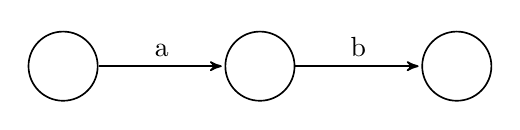
\begin{tikzpicture}[->,>=stealth',shorten >=1pt,auto,node distance=2.5cm,
                    semithick]
  \tikzstyle{every state}=[fill=none,text=black]

  \node[state] (1) {$$};
  \node[state] (2) [right of=1] {$$};
  \node[state] (3) [right of=2] {$$}; 
  
  \path 	(1)	edge node {a} (2)
  		(2)	edge node {b} (3);
\end{tikzpicture} 
\end{minipage}% 
=
\begin{minipage}{.5\textwidth}
\centering
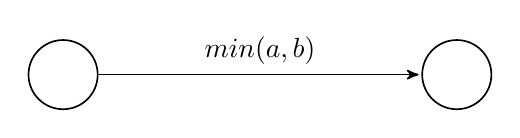
\begin{tikzpicture}[->,>=stealth',shorten >=1pt,auto,node distance=5cm,
                    semithick]
  \tikzstyle{every state}=[fill=none,text=black]

  \node[state] (1) {$$};
  \node[state] (2) [right of=1] {$$};
  
  \path 	(1)	edge node {$min(a, b)$} (2);
\end{tikzpicture} 
\end{minipage}

\subsubsection{Networks with multiple sources and sinks}
A maximum flow problem may have several sources and sinks, rather than just one of each. To fix that, we just add a supersource and a supersink with infinity capacity from $s$ to each of the multiple sources.
%%
\subsection{The Ford-Fulkerson Method}

\begin{algorithm}
\begin{algorithmic}[1]
\State{FORD-FULKERSON-METHOD}{$(G,s,t)$}
   \State initialise flow $f$ to $0$
   \While{there exists an augmenting path $p$ in the residual network $G_f$}
      \State augment flow $f$ along $p$
   \EndWhile
   \State \textbf{return} $f$
\end{algorithmic}
\end{algorithm}
%%
\subsubsection{Residual Network}
Suppose that we have a flow network $G = (V, E)$ with source $s$ and sink $t$. Let $f$ be a flow in $G$, and consider a pair of vertices $u, v \in V$. We define the residual capacity $c_f(u, v)$ by

\[
 c_f(u,v) =
  \begin{cases}
  	c(u,v) - f(u,v) & \text{if } (u,v) \in E, \\
  	f(v,u) & \text{if } (v,u) \in E, \\
  	0 & \text{otherwise}
  \end{cases}
\]

\subsubsection{Augmenting paths}
\subsubsection{Cuts of Flow Networks}
\subsubsection{The basic Ford-Fulkerson Algorithm}
\subsubsection{Analysis of Ford-Fulkerson}
\subsubsection{The Edmond-Karp Algorithm}

\subsection{Maximum bipartite matching}
\subsubsection{The Maximum-bipartite-mathing problem}
\subsubsection{Finding a maximum bipartite matching}

\newpage

\section{Fibonacci Heaps}
\newpage

\section{NP-Completeness}
\newpage

\section{Randomised Algorithms}
\newpage

\section{Exact Exponential Algorithms}
\newpage

\section{Approximation Algorithms}
\newpage

\section{Computational Geometry}
\newpage

\section{Linear Programming and Optimisation}

%-----------------------------------------------------------------------------
\end{document}